\documentclass[12pt, leqno]{article} %% use to set typesize 
\usepackage{amsfonts}
\usepackage{amsmath}
\usepackage{amssymb}
\usepackage{fancyhdr}
\usepackage{hyperref}
\usepackage{tikz}
\usepackage{pgfplots}
\usepackage{listings}

\newcommand{\bbR}{\mathbb{R}}
\newcommand{\bbC}{\mathbb{C}}
\newcommand{\calV}{\mathcal{V}}
\newcommand{\calW}{\mathcal{W}}
\newcommand{\ddiag}{\operatorname{diag}}
\newcommand{\fl}{\operatorname{fl}}
\newcommand{\macheps}{\epsilon_{\mathrm{mach}}}
\newcommand{\matlab}{\textsc{Matlab}}

\newcommand{\hdr}[2]{
  \pagestyle{fancy}
  \lhead{Bindel, Spring 2016}
  \rhead{Numerical Analysis (CS 4220)}
  \fancyfoot{}
  \begin{center}
    {\large{\bf Notes for #1}}
  \end{center}
  \lstset{language=matlab,columns=flexible}  
}

\usepackage{hyperref}

\begin{document} \phdr{Proj 2: Where Are My Glasses?}

\begin{figure}
\begin{center}
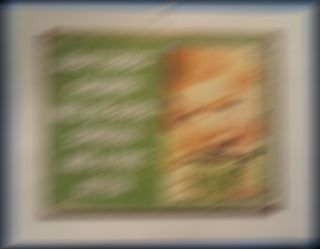
\includegraphics[width=0.5\textwidth]{proj2code/blurry.png}
\end{center}
\caption{A blurred mystery photo taken at the Ithaca SPCA.}
\label{fig1}
\end{figure}

\section{Introduction}

The image in Figure~\ref{fig1} is a blurred version of a picture that
I took at the local SPCA.  Your mission is to try three approaches to
de-blurring this picture, and to analyze why these approaches behave
as they do.

Images in MATLAB are represented as three-dimensional arrays of size
height $\times$ width $\times$ 3, where the three layers represent the
red, green, and blue color intensities at each pixel.  The blurred
image file in Figure~\ref{fig1} has eight-bit color depth, which means
that each of the RGB values is represented as an integer between $0$
and $255$ (inclusive).  For convenience, we will reshape these
three-dimensional arrays into matrices with height $\times$ width rows
and three columns, with the columns representing red, green, and blue
color intensities as floating point numbers (still between 0 and 255).

The image was constructed from the original picture by the MATLAB
commands
\begin{lstlisting}
  h = fspecial('motion', 30, 25);
  im1 = imread('origimg.jpg');
  im2 = imfilter(im1, h);
  imwrite(im2, 'blurry.png');
\end{lstlisting}
These commands simulate motion blur at an angle of 25 degrees over a
line about 30 pixels long.  This is a {\em linear} transformation;
that is, we can write
\[
  V^{\mathrm{blur}} = \operatorname{round}(H V^{\mathrm{orig}})
\]
where 
\[
  V^{\mathrm{orig}} = 
  \begin{bmatrix} 
    v^{\mathrm{orig}}_{\mathrm{red}} &
    v^{\mathrm{orig}}_{\mathrm{green}} &
    v^{\mathrm{orig}}_{\mathrm{blue}}
  \end{bmatrix}
\]
and $V^{\mathrm{blur}}$ has a similar layout.  Here the function
$\operatorname{round}(\cdot)$ means rounding each color intensity to
eight bits (i.e. to an integer between $0$ and $255$).  If everything
were done exactly (no noise and no rounding to eight bits), we could
recover the original image by computing $H^{-1} V^{\mathrm{blur}}$.
Of course, then this would not be much of a project!

You are given the following files:
\begin{description}
\item[{\tt blurry.png}]: Blurred image file.
\item[{\tt p2setup.m}]: Loads the image and forms the blurring matrix $H$.
\item[{\tt p2image.m}]: Displays an image (loaded or reconstructed).
\item[{\tt p2runner.m}]: Runs the three methods, saves images, and reports run times.
\end{description}
You are responsible for the following deliverables:
\begin{itemize}
\item Four MATLAB functions to implement the deblurring methods.
\item A report that addresses the questions posed in the rest of this prompt.
\end{itemize}
This project is inspired by the project on image deblurring by James
G. Nagy and Dianne P. O'Leary (``Image Deblurring: I Can See Clearly
Now'' in {\em Computing in Science and Engineering}; Project: Vol. 5,
No. 3, May/June 2003, pp. 82-85; Solution: Vol. 5, No. 4, July/August
2003, pp. 72-74).  As usual, you are welcome to use any ideas or code
you find in the literature, including in the article by Nagy and
O'Leary, provided you give an appropriate citation.


\section{The approaches}

\subsection{The naive approach}

The simplest reconstruction approach is to simply solve
\[
  V^{\mathrm{naive}} \approx H^{-1} V^{\mathrm{blur}}.
\]
You should complete the following function to implement this approach:
\begin{lstlisting}
  function imresult = p2naive(imblurd, H)
\end{lstlisting}

\paragraph*{Questions}
\begin{enumerate}
\item
  What does the reconstructed image look like?  You can use the
  function {\tt p2image} to see a picture.
\item
  For this image, give an estimated bound on
  $\|HV^{\mathrm{orig}}-V^{\mathrm{blur}}\|_F/\|V^{\mathrm{blur}}\|_F$,
  and use the MATLAB function {\tt condest}\footnote{{\tt condest}
    computes the condition number in the 1-norm rather than the
    2-norm, but the order of magnitudes are similar.}
  to estimate the condition
  number of $H$.  Use these estimates to explain the picture.
\end{enumerate}

\subsection{Tikhonov regularization}

A better approach to deblurring the image is {\em Tikhonov
  regularization}:
\[
  V^{\mathrm{tik}} = 
  \operatorname{argmin}_V \|HV-V^{\mathrm{blur}}\|_F^2 + \beta^2 \|V-V^{\mathrm{blur}}\|_F^2.
\]
You should complete the following function to implement this approach:
\begin{lstlisting}
  function imresult = p2tikhonov(imblurd, H, beta)
\end{lstlisting}
The regularization parameter $\beta$ should be small (in order that
the data mismatch term $\|HV-V^{\mathrm{blur}}\|_F^2$ should be
small); but it should not be so small that the regularized problem
still has the conditioning problems of the naive approach.  How to
choose the regularization parameter is in general an interesting
problem, but one we will leave for another day.  For this particular
example, $\beta = 10^{-2}$ does a pretty good job.

\paragraph*{Questions}
\begin{enumerate}
\item
  Show that the Tikhonov regularized problem is equivalent to
  \[
  V^{\mathrm{tik}} = \operatorname{argmin}_V
  \left\| 
    \begin{bmatrix} H \\ \beta I \end{bmatrix} V -
    \begin{bmatrix} V^{\mathrm{blur}} \\ \beta V^{\mathrm{blur}} \end{bmatrix}
  \right\|_F^2
  \]
\item
  Write an analytic formula for the singular values of the regularized
  matrix
  \[
    \begin{bmatrix} H \\ \beta I \end{bmatrix}
  \]
  in terms of $\beta$ and of the singular values $\sigma_1, \ldots,
  \sigma_N$ for $H$.  The largest singular value of $H$ is just below
  one; using this fact, together with the condition number estimated
  earlier, give an estimate of the size of the smallest singular value
  for this matrix in the case of $\beta = 10^{-2}$.
\item
  What would be the complexity of solving this ordinary least
  squares system using dense QR factorization?
  Fortunately, we do not need to use dense factorization to solve this
  problem.  I recommend using the sparse QR factorization in MATLAB;
  do {\tt help qr} to learn more.  Or you can just use backslash!
\end{enumerate}

\subsection{Landweber iteration}

The {\em Landweber iteration} is a fixed point iteration of the form:
\begin{equation}
  V^{(k+1)} = V^{(k)} + \alpha H^T (V^{\mathrm{blur}}-H V^{(k}).
  \label{eq:landweber}
\end{equation}
For $\alpha$ sufficiently small, $V^{(k)} \rightarrow V^{(\infty)}$ as
$k \rightarrow \infty$, where $H^T H V^{(\infty)} = H^T
V^{\mathrm{blur}}$.  Thus, we should {\em asymptotically} recover the
same solution generated by the naive approach.  However, we can
effectively regularize the problem by looking at {\em partly
  converged} results.  You should implement this approach in a MATLAB
function with the following signature:
\begin{lstlisting}
% imresult = p2landweber(imblurd, H, n, alpha)
%
% Deblur the image using the Landweber iteration
% for n steps, starting from the blurred image.

function imresult = p2landweber(imblurd, H, n, alpha)
\end{lstlisting}

\paragraph*{Questions}

\begin{enumerate}
\item
  Show that the fixed point iteration (\ref{eq:landweber}) converges whenever
  \[
    0 < \alpha < \frac{2}{\sigma_1^2},
  \]
  where $\sigma_1$ is the largest singular value of $H$.

  Computing $\sigma_1^2$ can be expensive, but there is a cheap upper
  bound:
  \[
  \sigma_1^2 \leq \|H\|_1 \|H\|_{\infty}.
  \]
  In this particular case, $\|H\|_1 = \|H\|_{\infty} = 1$ and
  $\sigma_1^2$ turns out to be just a smidge less than one.

\item
  My script uses a default value of $\alpha = 2$.  Play with this
  parameter.  Do you get better results for other values?
\item
  My test script ({\tt p2runner}) simply runs for 100 iterations.
  Build an alternate version of {\tt p2landweber} that shows the
  images at each intermediate step of the iteration.  At what step are
  you first able to read the text?  You don't need to include your
  code, but ideally your writeup should include a picture of the
  reconstruction at the relevant step.
\item
  Compare the run time and image quality for the Landweber iteration
  for this problem (with $\alpha = 2$ and 100 iterations) to the 
  Tikhonov regularized computation (using MATLAB's sparse direct QR
  solver).
\end{enumerate}

\subsection{LSQR iteration}

The {\em LSQR iteration} is a Krylov subspace iteration that minimizes
the residual for least squares problems or ill-posed linear systems.
Like the Landweber iteration, LSQR tends to have a regularizing effect
when it is not run all the way to convergence.  MATLAB has an LSQR
solver built in (type {\tt help lsqr}), which you should use to
implement the following function.
\begin{lstlisting}
% imresult = p2landweber(imblurd, H, n)
%
% Deblur the image using the LSQR iteration for n steps.

function imf = p2lsqr(imblurd, H, n)
\end{lstlisting}
You will need to make three calls to {\tt lsqr}, one per column of
{\tt imblurd}.  You will probably want to specify a tolerance and
a maximum iteration count.  I recommend choosing a tolerance of
$10^{-6}$ -- you won't reach this tolerance within a hundred
iterations, but this doesn't matter so much. There is currently no
LSQR implementation in Octave, so we recommend that you use
the implementation by Paige and Saunders:
\url{http://web.stanford.edu/group/SOL/software/lsqr/}

\paragraph*{Questions}

\begin{enumerate}
\item
  Compare the run time, image quality, and residual error (measured in
  Frobenius norm) for LSQR as compared to Landweber with $\alpha = 2$.
  Comment on what you see for 30 iterations and for 100 iterations.
\end{enumerate}

\section{Notes}

\begin{enumerate}
\item
  The type of very ill-conditioned problems seen here occur frequently
  not only in image reconstruction and inverse problems, but also in
  solving ``first kind'' integral equations that occur in mathematical
  physics.  Integral equations of the second kind tend to be much
  better behaved.
\item
  The Landweber iteration also works for ordinary least squares
  problems in which the matrix is tall and thin (rather than
  square problems of the sort described here).
\item
  One of the advantages of the Landweber and LSQR iterations which we have
  not highlighted in this assignment is that we do not actually need
  the matrix $H$ in any explicit form.  We only need the ability to
  multiply by $H$ and $H^T$.  This is particularly useful in medical
  imaging problems, where $H$ can often be efficiently applied via
  fast Fourier transforms.
\end{enumerate}

\end{document}
